\section{Results} \label{sec:results}

\subsection{Logistic regression}
\iffalse
\begin{figure} [H]
	\centering
	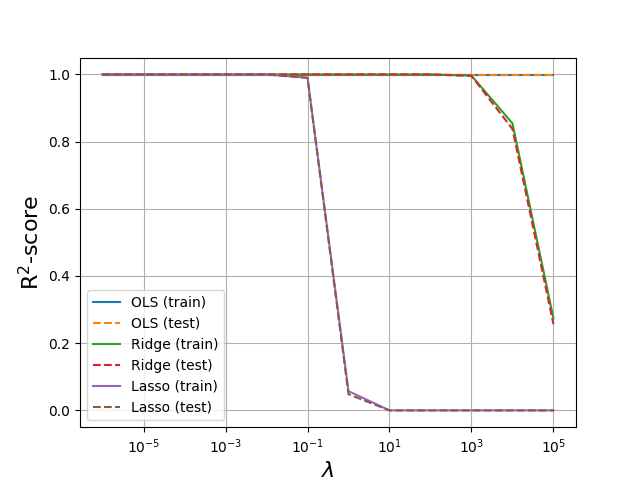
\includegraphics[scale=0.65]{../plots/lambda_vs_R2_linear.png}
	\caption{The R$^2$-score as a function of the penalty. }
	\label{fig:lambda_vs_R2_linear}
\end{figure} 
\fi

\begin{table} [H]
	\caption{Accuracy, softmax output}
	\begin{tabularx}{\textwidth}{c|XX:XX:XX:XX} \hline\hline
		\label{tab:logistic}
		\textbf{Epochs}& \multicolumn{8}{c}{\textbf{Regularization}}\\ \hline
		&\multicolumn{2}{c}{0.1}&\multicolumn{2}{c}{0.001}&\multicolumn{2}{c}{0.00001}&\multicolumn{2}{c}{0}\\ \hline
		& Train & Test & Train & Test & Train & Test & Train & Test\\ \hline
		10 & 0.3925 & 0.4112 & 0.2000 & 0.2042 & 0.2543 & 0.2447 & 0.2308 & 0.2429\\
		20 & 0.4572 & 0.4802 & 0.2927 & 0.2843 & 0.3320 & 0.3238 & 0.4135 & 0.3919\\
		30 & 0.5741 & 0.5842 & 0.2948 & 0.2815 & 0.3387 & 0.3395 & 0.4393 & 0.4186\\
		40 & 0.5780 & 0.5603 & 0.2948 & 0.2861 & 0.3433 & 0.3385 & 0.4402 & 0.4103\\
		50 & 0.5916 & 0.5998 & 0.3007 & 0.2833 & 0.3389 & 0.3395 & 0.4590 & 0.4453\\ \hline\hline
	\end{tabularx}
\end{table}

\subsection{Feed-forward Neural Networks}
\begin{table} [H]
	\caption{Accuracy, sigmoid function was used in hidden layers, softmax on output. Dropout was used.}
	\begin{tabularx}{\textwidth}{c|XX:XX:XX:XX} \hline\hline
		\label{tab:fnn}
		\textbf{Epochs}& \multicolumn{8}{c}{\textbf{Hidden nodes}}\\ \hline
		&\multicolumn{2}{c}{1024}&\multicolumn{2}{c}{2x1024}&\multicolumn{2}{c}{3x1024}&\multicolumn{2}{c}{4x1024}\\ \hline
		&Train&Test&Train&Test&Train&Test&Train&Test\\ \hline
		20& 0.8684 & 0.8464 & 0.8603 & 0.8602 & 0.8541 & 0.8602 & 0.8341 & 0.8298\\
		40& 0.9245 & 0.8924 & 0.9204 & 0.8942 & 0.9195 & 0.8868 & 0.8990 & 0.8924\\
		60& 0.9416 & 0.9062 & 0.9508 & 0.9154 & 0.9317 & 0.9016 & 0.9254 & 0.8960\\
		80& 0.9572 & 0.8942 & 0.9556 & 0.9163 & 0.9508 & 0.9172 & 0.9418 & 0.9016\\
		100& 0.9607 & 0.9016 & 0.9579 & 0.9126 & 0.9627 & 0.9181 & 0.9510 & 0.9200\\ \hline\hline
	\end{tabularx}
\end{table}

We could go further and increase the number of epochs. With 3x1024 hidden nodes and 1000 epochs, we were able to get an accuracy of 0.99 for the training set and 0.94 for the test set. 

\subsection{Convolutional Neural Networks}
\begin{table} [H]
	\caption{}
	\begin{tabularx}{\textwidth}{c|XXXX} \hline\hline
		\label{tab:cnn}
		\textbf{Epochs}& \multicolumn{4}{c}{\textbf{Hidden nodes}}\\ \hline
		&1024&2x1024&3x1024&4x1024\\ \hline
		
		100& 0.4371 & 0.4381 & 0.3333 & \\
		200& 0.4379 & 0.4367 & 0.3333 & \\
		300& 0.4371 & 0.4382 & 0.3333 & \\
		400& 0.9930 & 0.9929 & 0.9655 & \\
		500& 0.9935 & 0.9934 & 0.9679 & \\ \hline\hline
	\end{tabularx}
\end{table}

\subsection{Recurrent Neural Networks}
\begin{table} [H]
	\caption{}
	\begin{tabularx}{\textwidth}{c|XXXX} \hline\hline
		\label{tab:rnn}
		\textbf{Epochs}& \multicolumn{4}{c}{\textbf{Hidden nodes}}\\ \hline
		&1024&2x1024&3x1024&4x1024\\ \hline
		
		100& 0.4371 & 0.4381 & 0.3333 & \\
		200& 0.4379 & 0.4367 & 0.3333 & \\
		300& 0.4371 & 0.4382 & 0.3333 & \\
		400& 0.9930 & 0.9929 & 0.9655 & \\
		500& 0.9935 & 0.9934 & 0.9679 & \\ \hline\hline
	\end{tabularx}
\end{table}
